\documentclass{whutmod}
\usepackage{metalogo}
\usepackage{float}
\usepackage{subfigure} 
\usepackage{url}
\usepackage[style=caspervector,backend=biber,utf8]{biblatex}
\addbibresource{wenxian.bib}
\team{23}
\membera{刘子川}
\joba{编程}
\memberb{程宇}
\jobb{建模}
\memberc{陈荣兴}
\jobc{建模}
\hypersetup{
	colorlinks=true,
	linkcolor=black
}

\title{第四次论文格式}
\tihao{4} 

\begin{document}

%	\maketitle
	
	\begin{abstract}
“拍照赚钱”APP 是基于移动互联网的自助式劳务众包平台,使得企业可利 用大众力量,低成本、高效率地完成各种商品检查与信息搜集的任务。本文通过 建立数学模型,就 APP 中的任务定价问题进行分析,给出最优的任务定价方案。
   ~\\%~\\为换行
   
针对问题一, 针对问题的这一段总结。利用什么软件+建立什么模型+算法方法+求解的特点+主要的结果+评价及其推广。  注意黑体字\text{描黑重点关键词}。
~\\

针对问题二,对项目的任务定价规律进行\textbf{定性与定量研究}。利用 Matlab 的 cftool 工具箱绘制出任务的经纬度坐标与定价数据的\textbf{三维拟合图},观察到任务 分布密集的地区任务定价较低。对任务的位置数据进行空间离散化处理和 K-Means 分析,将任务分布的区域等划分为若干网格区域,定义影响任务定价的 四个因子,即网格内任务数量、会员人数、会员平均完成能力、任务与中心点的 距离。运用灰色关联矩阵定量分析四个影响因子与定价的相关度,分别为 0.9710,0.9671,0.9633,0.9390。得出所定义的指标对定价相关性很高,能较好 描述定价规律。最后通过比较未完成任务与已完成任务的相关度矩阵得出距离对 任务的完成的影响是最显著的


针对问题三,
   ~\\
   
针对问题四,
   ~\\

本文中所提到的模型优点主要有两点:一、在与污染源头距离较短时预测抗噪能力较强;二、利用更高定位精度和鲁棒性的直线解析法,溯源追踪能力较强。
  
\keywords{对流扩散方程\quad  直线解析法\quad  溯源算法\quad 拉普拉斯变换\quad }
		
	\end{abstract}
	
	%目录
	\tableofcontents
	\newpage	%换页符
	
	\section{问题重述}	
	\subsection{问题背景}
现代管理中,彼得德鲁克提出了"人力资源"的概念并认为"人力资源是与其他资源不一样的特殊资源",人力资源的其中一个特质是其具有自主流动性。根据勒温的场论,人才会根据自身需求与环境的适应性而做出离开或者留在某个环境的决定。人才是一个城市保持竞争活力和创新力的关键,在世界各国和全国各地积极推出人才吸引的政策背景下,一个地区的人才吸引力的核心内涵就是这个地区所具有的可以影响人才选择的能力。

全面、科学、系统地评价一个城市的人才吸引力是制定人才吸引计划的前提,城市人才吸引评价指标的选取受多方面影响,关键是要符合人才的理想,满足人才的需求和愿望。按照重要程度,人才的需求可以分为发展前景,收入和环境。发展前景是首要关心的因素,收入是人才流动的另一关键因素,环境因素包括治安、交通、污染、教育、医疗、购物等,也都是会考虑的因素。




	
	\subsection{问题提出}
围绕城市地区人才吸引力水平,以城市多指标评价体系为依据,依次提出以下问题:
		 
	\begin{itemize}
	\item [(1)] 根据数学模型及收集的数据,定量地分析武汉市的人才吸引力水平,并就武汉市的人才政策对人才吸引力水平的影响作出定量评价。
	\item [(2)] 结合人才类别,针对不同类型的人才,深入分析比较武汉市与其他同类城市在人才吸引力上的优势与不足,并给出有效提升人才吸引力的可行方案。
	\item [(3)] 结合模型结果及分析,给武汉市人力资源管理部分写一篇建议报告,要求论点明确,论据充分。
	\end{itemize}
	
	\section{模型假设}
	\begin{itemize}
		\item [(1)] 就写假设就行了吧
		\item [(2)] 
		\item [(3)]
		\item [(4)]
	\end{itemize}
	
	
	\section{符号说明}
%	每行都有线的表
%	\begin{center}
%		\begin{tabular}{cc}
%			\hline
%			\makebox[0.3\textwidth][c]{符号}	&  \makebox[0.4\textwidth][c]{意义} \\ \hline
%			$C_{0}$	    &  污染源初始浓度 \\ \hline
%			$C(x,t)$	    &  污染浓度随时空变化 \\ \hline
%			$u_{x}$	    &  江河平均纵向流速 \\ \hline
%			$E_{x}$  &  铊在江河纵向弥散系数\\ \hline
%		$p$   &  面污染物纵向距离\\ \hline
%			$K_{c}$	    & 污染物降解系数  \\ \hline
%		    $a$	& 污染超标系数 \\ \hline
%		     $x$	& 距污染源的一维距离 \\ \hline
%		      $t$	& 距污染发生后的时间 \\ \hline
%		       $V_{A}$	& 溶液摩尔体积 \\ \hline
%		      $M_{B}$	& 江水的摩尔质量 \\ \hline
%		     $\mu_{B}$	& 溶剂的粘度 \\ \hline		      
%		\end{tabular}
%	\end{center}

%三线表
	\begin{table}[H]
	\label{biao} \centering
		\begin{tabular}{cccc}
			\toprule[1.5pt]
			\multicolumn{1}{m{4cm}}{\centering 符号} & \multicolumn{1}{m{4cm}}{\centering 说明} & \multicolumn{1}{m{4cm}}{\centering 单位}\\
			\midrule[1pt]
			$C_{0}$	 &  污染源初始浓度 & 单位\\ 
			$C(x,t)$ &  污染浓度随时空变化 & 单位\\ 
			$u_{x}$	 &  江河平均纵向流速 & 单位\\ 
			$E_{x}$  &  铊在江河纵向弥散系数& 单位\\ 
			\bottomrule[1.5pt]
		\end{tabular}
	\end{table}

	\section{问题一模型的建立与求解}
	\subsection{问题的描述与分析}
	针对问题一,本题要求对武汉的人才吸引力做出量化评价,本文采用因子分析法建立模型,将通过不同的因子对变量的影响程度进行分析,建立客观的评价模型。首先根据题目要求和以往人才吸引要素研究,寻找合适的人才吸引力因素,确立要素框架并寻找各个因素相对应的数据。在将所得数据进行标准化与归一化处理后,进行$KMO$检验和巴特利特检验以验证所选变量是否适合做因子分析。通过主成分分析法确定公因子数目,求解旋转后因子荷载矩阵并对公因子命名。

%	\begin{figure}[H]
%		\centering
%		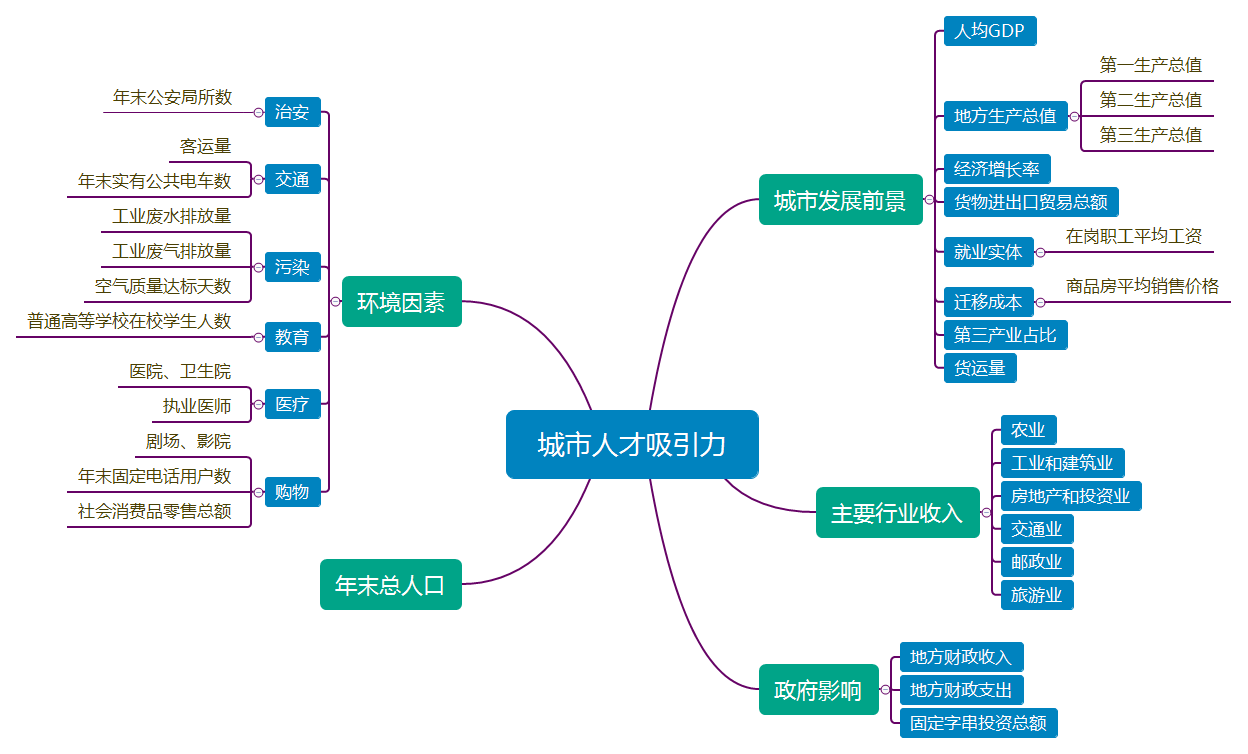
\includegraphics[width=.8\textwidth]{figures/clt.png}
%		\caption{算法流程图}\label{lct}
%	\end{figure}

		\subsection{预备工作}
		\subsubsection{评价指标体系构建}
		参考国家统计局对人才标准的划分,此处对人才的界 定是指,具有大专及以上学历的人员,以及具有初级以上 专业技术职称的人员或在专业技术岗位上工作的人员。
		
		在构建武汉市人才吸引力评价指标体系时,在指标方面,若选取总量太多,在评价模型时太为复杂,可行性低,若数据太少则评 价不够准确,脱离实际性。因此为尽可能客观反映吸引力,我们在遵循建立指标体系的科学性、系统性、可操作性、可比性原则, 参考大量文献,并兼顾总量指标和相对指标,选取城市发展前景、主要行业收入、政府影响、环境因素、年末总人口共5个二级指标和33个三级指标。具体指标体系如图~\ref{lct}~所示: 	
		\begin{figure}[H]
			\centering
			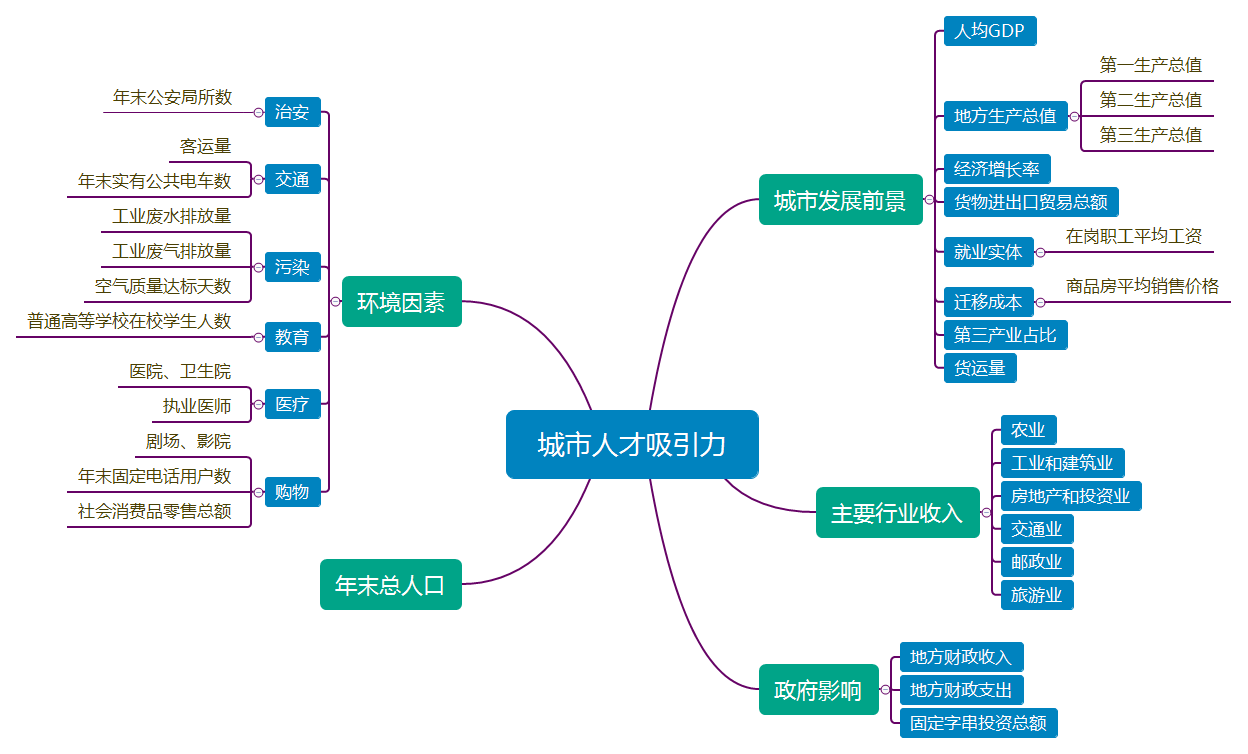
\includegraphics[width=\textwidth]{figures/clt.png}
			\caption{城市人才吸引力指标体系}\label{lct}
		\end{figure}  
		
		\subsubsection{基于因子分析的人才吸引力评价分析}
		\paragraph{同向化处理}
		~\\ 
		在评价城市人才的指标中,工业废水废气排放量和商品房平均销售价格不是越高越好,为方便比较,对这三个指标进行同向化处理, 公式如下:
		~\\ 同向指标 =-| 原始指标 - 原始指标的平均值 |
		\paragraph{标准化处理}
		~\\
		为了对变量进行比较并消除由于观测量纲的差异及数量级差异所造成的影响,将样本观测数据进行标准化处理,使标准化的变量均值为$0$,方差为$1$。其处理方法如下:
		\begin{gather}
		Z=\frac{X-\overline{X}}{\delta_{X}}
		\end{gather}
		式中:$\overline{X}$为$X$的期望值,$\delta_{X}$是$X$的标准差

	\subsection{模型的建立与求解}
	\subsubsection{公因子的确定}
	标准化后数据如表一所示(附表一),表一相关系数矩阵$R$如下(附加相关系数矩阵)
	设$\lambda_{1} \geqslant \lambda_{2} \geqslant \cdots \geqslant \lambda_{p}$为样本相关系数矩阵$R$的特征值,$??$为相应的标准正交化特征向量。设$m<p$,则因子载荷矩阵$\Lambda$为
	\begin{gather}
	\Lambda=\left[\sqrt{\lambda_{1}} \eta_{1}, \sqrt{\lambda_{2}} \eta_{2}, \cdots, \sqrt{\lambda_{m}} \eta_{m}\right]
	\end{gather}
    用$\boldsymbol{R}-\boldsymbol{\Lambda} \boldsymbol{\Lambda}^{\mathrm{T}}$对角元来估计特殊因子的的方差
	\begin{gather}
	\sigma_{i}^{2}=1-\sum_{j=1}^{m} \alpha_{i j}^{2}
	\end{gather}
	得总方差解释如表三(附表三)
	由表$3$特征根知,因子$1$的特征值$λ1=$,占方差的 $\%$。由图$1$知,当提取$1,2$个公因子时,特征值变化非常明显,当提取第$n+1$个以后的公因子时,特征值变化比较小,基本趋于平缓。由此说明,提取$n$个公因子对原变量信息的刻画有显著作用。因此,在这里我们提取$n$个公共因子,这$n$个公因子的累计方差达到$\%$,即这$n$个公因子可以反映原来$?$个指标的$???\%$的信息量,可见采用前$n$个公因子对武汉$2013~2017$年人才吸引力进行评价是比较合适的。
	\subsubsection{未转轴的因子载荷矩阵}
	表 4 中的每个数据表示了相应因子变量对相应原变量的相对重要程度。由于得到的公共因子与各指标的载荷分布归类比较困难,需要对因子载荷矩阵进行正交旋转,这里运用方差最大正交旋转法,得到旋转后的因子载荷矩阵表(4)。
	表$3$是初始因子载荷矩阵,由此可写出因子分析模型的如下:
	\begin{gather}
	\begin{array} { l } { \mathrm { X } _ { 1 } = 0.910 \mathrm { F } _ { 1 } - 0.193 \mathrm { F } _ { 2 } - 0.362 \mathrm { F } _ { 3 } - 0.062 \mathrm { F } _ { 4 } } \\ { \mathrm { X } _ { 2 } = 0.973 \mathrm { F } _ { 1 } - 0.021 \mathrm { F } _ { 2 } - 0.211 \mathrm { F } _ { 3 } - 0.092 \mathrm { F } _ { 4 } } \\ { \ldots \ldots } \\ { \mathrm { X } _ { 33 } = 0.859 \mathrm { F } _ { 1 } + 0.350 \mathrm { F } _ { 2 } + 0.325 \mathrm { F } _ { 3 } - 0.182 \mathrm { F } _ { 4 } } \end{array}
	\end{gather}
	通过凯撒正态化最大方差法,旋转在$?$次迭代后已收敛。得表$5$(附表五)
	
	根据表 5 发现,旋转后的因子系数已经明显向两极分化,有了更鲜明的实际意义。因子载荷的绝对值越大,则表明该因子与变量的重叠性越高,在解释因子的时候就越重要。
	(因子命名)
	\subsubsection{求得因子得分和综合绩效得分}
	采用回归法估计因子得分系数,并输出因子得分系数矩阵。具体结果见表$6$
	由估计出的因子得分,可以量化描述城市人才吸引力水平,利用因子得分可以从不同角度对城市人才吸引力水平进行比较分析。为了便于对各城市进行人才吸引力评价,现利用武汉每年度的因子得分表计算综合得分,吸引力水平的获取是基于总方差分解表中旋转后各因子的方差贡献率及计算所得的城市各因子得分获取的。其计算公式如下:
	\begin{gather}
	\mathrm { F } = \left( 60.154 \mathrm { F } _ { 1 } + 16.857 \mathrm { F } _ { 2 } + 16.817 \mathrm { F } _ { 3 } + 6.171 \mathrm { F } _ { 4 } \right) / 100
	%(附结果计算公式)
	\end{gather}
	计算结果见表$7$
	\subsection{结果分析}


%	\parencite{geng2019novel}为文献引用
	查阅资料可得\parencite{宋鸿2010城市人才吸引力的影响因素及提升对策}
	
%	~\ref{llllll}~为图表引用,中间为为图表\label{}
具体浓度分布如图~\ref{llllll}~所示:


	\section{问题二模型的建立与求解}
	\subsection{问题的描述与分析}
%	问题分析写\textbf{流程图!!}其流程图如图~\ref{lct}~所示:
%			\begin{figure}[H]
%	\centering
%	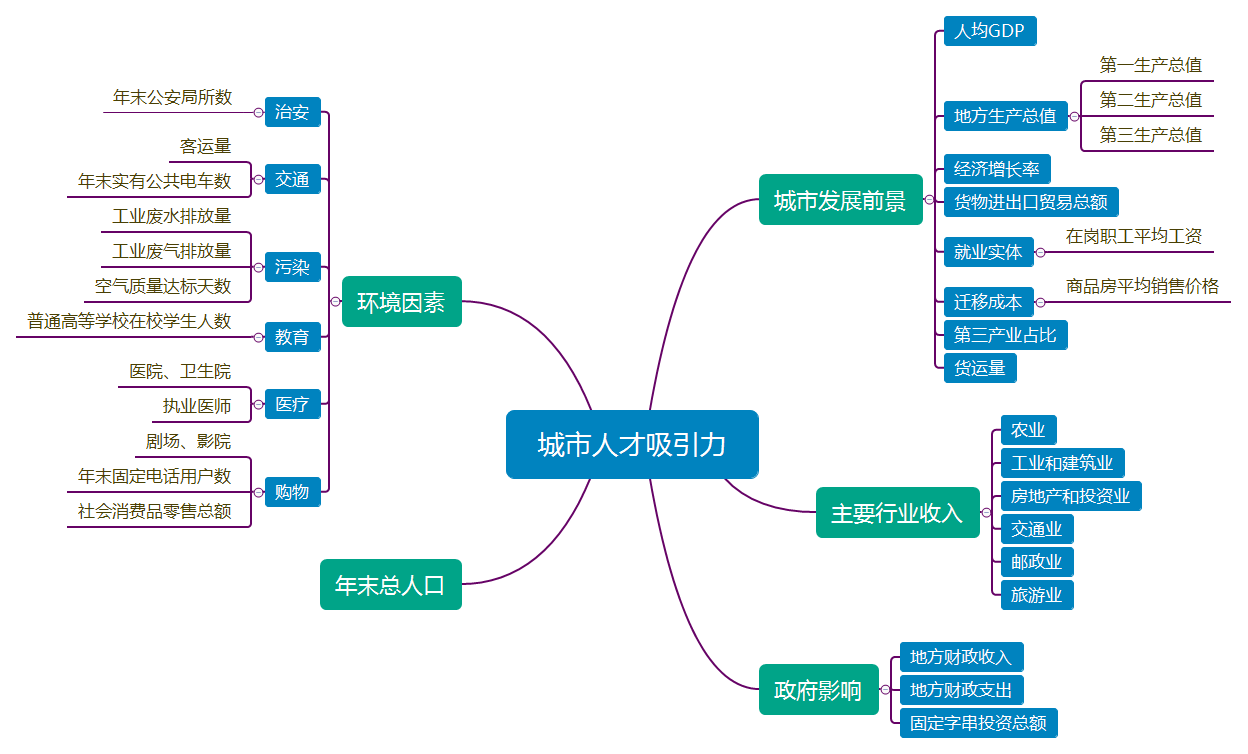
\includegraphics[width=.8\textwidth]{figures/clt.png}
%	\caption{算法流程图}\label{lct}
%	\end{figure}
	\subsection{模型的建立与求解}
	

	\section{问题三模型的建立与求解}
	
	
	\subsection{问题的描述与分析}

	\subsection{模型的建立与求解}


	\section{模型的评价}
	\subsection{模型的优点}
xxxxxxxxxxxxxxxxxxxxxxxxx
	
	\subsection{模型的缺点}
xxxxxxxxxxxxxxxxxxxxxxxxxxxxxx


	\subsection{模型的改进与展望}%
xxxxxxxxxxxxxxxxxxxxxxxxxxxx
	\newpage	%换页符
	%%参考文献
	%\begin{thebibliography}{9}%宽度9
	% \setlength{\itemsep}{-2mm}
	\nocite{*}		%排版未引用的参考文献
	\printbibliography[title = {参考文献}]	%使用国标参考文献添加方式
	%参考文献添加到wenxian.bib里,再引用
	
	\newpage
	%附录
	\appendix %%附录
\section{代码}
\subsection{爬取数据--python源代码}
\begin{lstlisting}[language=python]%这里修改语言
xxxxxxxxxxxxxxxxxxxxxxxxxxxxxxxx
\end{lstlisting}

\end{document}